%
% Master-File
%
%\documentclass[12pt,a4paper]{letter}
\documentclass[12pt,a4paper]{article}
%\documentclass[12pt,a4paper]{report}

\input{ighpreamble}     % definiert texeinstellungen und \newcommands

\usepackage{listings} % Code/Befehl-Listings (fp)
\usepackage{svn}

% Fette-Typewriter Font f�r Markierungen in Listings (fp)
\DeclareFontShape{OT1}{cmtt}{bx}{n}
{
  <5><6><7><8><9><10><10.95><12><14.4><17.28><20.74><24.88>cmttb10
}{}

% Konfiguration f�r "listings"-Paket (fp)
\lstset{basicstyle=\ttfamily\small,numberstyle=\tiny,aboveskip=4mm,
  belowskip=2mm,gobble=2,escapechar=`}

\newcommand{\version}{1.1.1}

%
% Hier als Entwurf kennzeichnen
%
%\entwurf{Draft}

\selectlanguage{english}

\begin{document}

%
% nachfolgendes bedarfsweise hereinnehmen
%

% Die  zwei Titelseiten:
%\ightitlepage{
%               Erste Zeile Titel\\[1ex]
%               Zweite Zeile Titel\\[1ex]
%               vielleicht dritte Zeile\\[1ex]
%               }{Musterfirma}{Monat 200X}
%
% alternativ f�r kurze Informationen
% Titel entsprechend aendern
%

\begin{titlepage}
  \begin{center}
    \Large

    \rule{\textwidth}{1.5mm}

    \Huge
    \raisebox{-0.8ex} {
\includegraphics[height=5ex]{etherlabsign-gr}}\\[3ex]
    \Large
    {\bf EtherLab\regTM/RTW\\[1ex]
      Version \version\\[1ex]}

    \vspace{1ex}
    \rule{\textwidth}{1.5mm}

    \vspace{18ex}

    \vspace{5ex}
    created by\\[1ex]
    Ingenieurgemeinschaft \IgH\\

    \vspace{\fill}
    \Large Essen\\[2ex]
    \today\\[2ex]
  \end{center}
\end{titlepage}

% R�ckseite des Deckblattes

\begin{titlepage}
  \vspace*{\fill}
  {\small
    Ingenieurgemeinschaft IgH\\
    Heinz-B�cker-Str. 34\\
    D-45356 Essen\\
    Tel.: +49-201-36014-0\\
    Fax.: +49-201-36014-14\\
    E-mail: igh@igh-essen.com}
\end{titlepage}

%\tecnote{Information}

%
% Das Inhaltsverzeichnis:
\ightoc
\newpage
%
% Das Abbildungsverzeichnis:
\ighfig
\newpage
%
% Das Tabellenverzeichnis:
%\ightab
%

% Der eigentliche Inhalt:
%
% Inhaltsfile
%
\rfoot{$Id$}

\begin{ighsec}{Introduction}
\label{sec:einleitung}

A blockset was created for the real time connection of EtherCAT\regTM\ 
components in MATLAB/Simulink\regTM. EtherCAT\regTM\ slaves can be
selected from the \texttt{etherlab\_lib} in MATLAB/Simulink/RTW\regTM\ 
and directly included into the model. After that, the model ist
translated to C code and compiled to a loadable Linux kernel module.

\end{ighsec}

%--------------------------------------------------------------------

\begin{ighsec}{Concept}
\label{sec:konzept}

EtherLab\regTM/RTW is a system to create controllers using
EtherCAT\regTM\ hardware, that run with the EtherLab\regTM\ 
EtherCAT\regTM\ master inside the Linux kernel. The user is able to
create models using the MATLAB/Simulink\regTM\ library
\texttt{etherlab\_lib}, that are compiled to a loadable Linux kernel
module by traversing Realtime Workshop and EtherLab\regTM/RTW.

The EtherLab\regTM/RTW package can be subdivided into the components
listed below:

\begin{itemize}
\item The \texttt{etherlab\_lib} for MATLAB/Simulink\regTM. It
  contains all necessary blocks for the creation of models with
  EtherCAT\regTM\ slaves.
\item The support code, that compiles a Linux kernel module of the
  output of Realtime Workshop. This happens in background and is not
  visible to the user.
\item The kernel module \texttt{rt\_kernel}, that is responsible for
  the real time execution of the created models. On loading, the
  modules register at the \texttt{rt\_kernel}.
\item The EtherLab\regTM\ ``Buddy Process'', that acts as a
  counterpart to the \texttt{rt\_kernel} in user space and is
  responsible for providing real time data in user space (see
  figure~\ref{fig:architektur}).
\end{itemize}

\begin{figure}[H]
  \begin{center}
    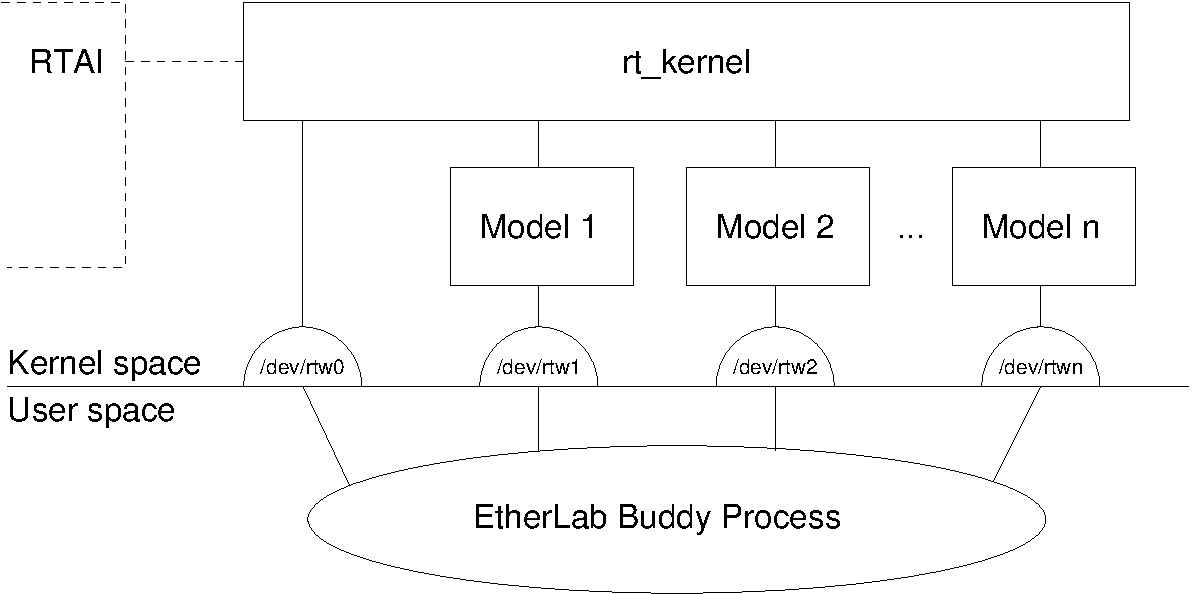
\includegraphics[width=\textwidth]{images/etl-arch}
    \caption{EtherLab\regTM\ architecture}
    \label{fig:architektur}
  \end{center}
\end{figure}

\end{ighsec}

%--------------------------------------------------------------------

\begin{ighsec}{Installation}
\label{sec:installation}

\begin{ighsec}{Prerequisites}

Prerequisites for the installation of EtherLab\regTM/RTW:

\begin{itemize}
\item Linux-Kernel 2.6 (including kernel sources)
\item RTAI $\ge$ 3.3
\item EtherLab\regTM\ EtherCAT\regTM\ Master 1.3.x
\end{itemize}

It is recommended to install EtherLab\regTM\ components to
\texttt{/opt/etherlab}. If this directory does not exist, it can be
created with the commands below:

\begin{lstlisting}
  # `\textbf{mkdir /opt/etherlab}`
  # `\textbf{chown root:users /opt/etherlab}`
  # `\textbf{chmod 775 /opt/etherlab}`
\end{lstlisting}

\end{ighsec}

\begin{ighsec}{Installation of EtherLab\regTM/RTW}
\label{sec:inst-paket}

Installation is done after copying the EtherLab\regTM/RTW tarball from
the EtherLab\regTM\ CD (or downloading from \url{etherlab.org}) as
normal user according to the commands below. The last command installs
EtherLab\regTM/RTW into the directory \texttt{/opt/etherlab/rtw}. A
different target directory can be selected via the \texttt{--prefix}
parameter of the \texttt{configure} script (see \texttt{configure
  --help}).

\begin{lstlisting}
  `\$` `\textbf{tar xzf etherlab\_rtw-\version.tar.gz}`
  `\$` `\textbf{cd etherlab\_rtw-\version/}`
  `\$` `\textbf{./configure}`
  `\$` `\textbf{make}`
  `\$` `\textbf{make install}`
\end{lstlisting}

\end{ighsec}

\begin{ighsec}{Installation of the EtherLab\regTM\ Blockset}
\label{sec:inst-blockset}

As a prerequisite for the \texttt{setup\_etherlab} command (see below)
to succeed, the file \textit{toolbox/local/pathdef.m} inside the
MATLAB\regTM\ installation directory must be writable for the user
running MATLAB\regTM. Enter the below commands (as \textit{root}) to
make it writable for all users in the group \textit{users} (substitute
the variable \textit{MATLABDIR} with the correct path first):

\begin{lstlisting}
  # `\textbf{chown :users \$MATLABDIR/toolbox/local/pathdef.m}`
  # `\textbf{chmod 664 \$MATLABDIR/toolbox/local/pathdef.m}`
\end{lstlisting}

To setup the EtherLab\regTM/RTW library \texttt{etherlab\_lib} for the
use in MATLAB\regTM, the below commands must be entered (out of
MATLAB\regTM).

\begin{lstlisting}
  >> `\textbf{cd /opt/etherlab/rtw}`
  >> `\textbf{setup\_etherlab}`
\end{lstlisting}

\end{ighsec}

\begin{ighsec}{Starting EtherLab\regTM/RTW as a Service}
\label{sec:dienst}

If EtherLab\regTM/RTW is to be started as a service, the provided init
script \texttt{etherlab} can be used. However, the insertion of the
service is dependent on the GNU/Linux distribution used. The command
sequence below is intended for SUSE Linux:

\begin{lstlisting}
  # `\textbf{cp /opt/etherlab/rtw/bin/etherlab /etc/init.d/}`
  # `\textbf{insserv etherlab}`
\end{lstlisting}

\end{ighsec}

\end{ighsec}

%--------------------------------------------------------------------

\begin{ighsec}{The EtherLab\regTM\ Library}
\label{sec:lib}

The EtherLab\regTM\ library \texttt{etherlab\_lib} was designed to
allow the creation of EtherLab\regTM\ models. It contains blocks for
all supported EtherCAT\regTM\ slaves. To show the library window (see
figure~\ref{fig:blockset}), the commands below have to be entered in
MATLAB\regTM:

\begin{lstlisting}
  >> `\textbf{bdclose all; set\_param(0, 'CharacterEncoding', 'ISO-8859-1')}`
  >> `\textbf{etherlab\_lib}`
\end{lstlisting}

The first line is only necessary on non-english systems to avoid
problems regarding character encoding.

Figure~\ref{fig:blockset} shows the window containing the
\texttt{etherlab\_lib} with the EtherCAT\regTM\ blockset. Each block
has a configuration dialog, that shows up after double-clicking on the
block area. There is a ``Help'' button in all of the configuration
dialogs, that provides detailed help concerning the dialog elements.

\begin{figure}[H]
  \begin{center}
    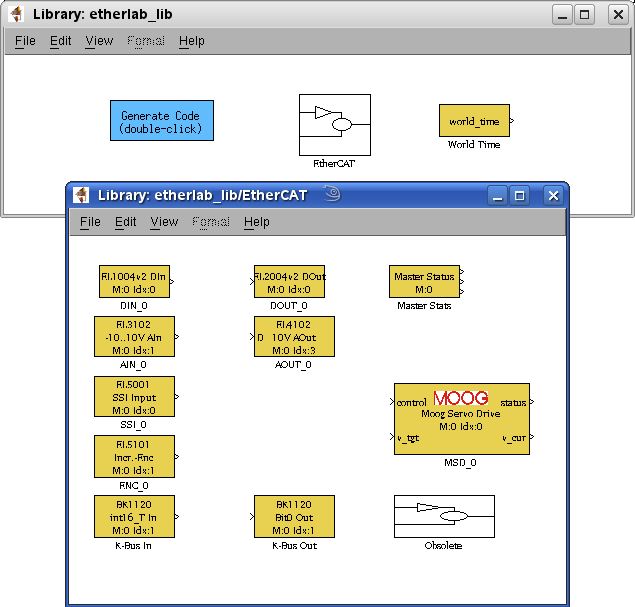
\includegraphics[width=0.9\textwidth]{images/blockset.png}
    \caption{EtherLab\regTM\ blockset}
    \label{fig:blockset}
  \end{center}
\end{figure}

Figure~\ref{fig:el10xx} shows the configuration dialog for the
digital-input slaves of the Beckhoff EL10XX series.

\begin{figure}[H]
  \begin{center}
    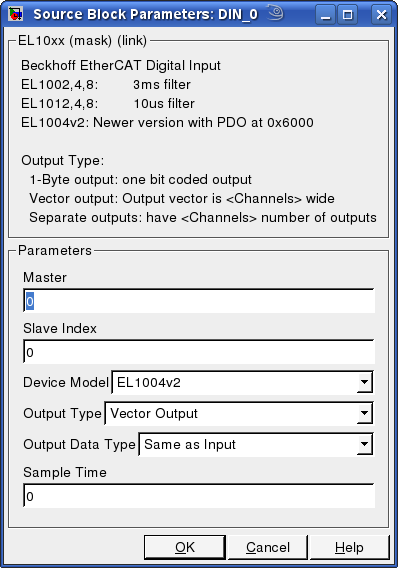
\includegraphics[width=0.4\textwidth]{images/el10xx.png}
    \caption{EL10xx configuration dialog}
    \label{fig:el10xx}
  \end{center}
\end{figure}

Figure~\ref{fig:el20xx} shows the configuration dialog for the
digital-output slaves of the Beckhoff EL20XX series.

\begin{figure}[H]
  \begin{center}
    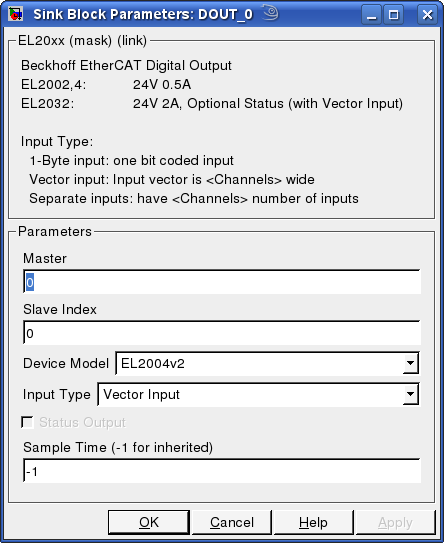
\includegraphics[width=0.4\textwidth]{images/el20xx.png}
    \caption{EL20xx configuration dialog}
    \label{fig:el20xx}
  \end{center}
\end{figure}

Figure~\ref{fig:el31xx} shows the configuration dialog for the
analog-input slaves of the Beckhoff EL31XX series.

\begin{figure}[H]
  \begin{center}
    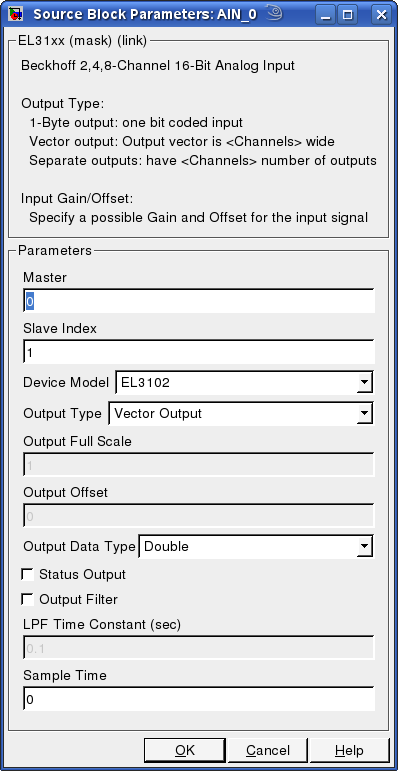
\includegraphics[width=0.4\textwidth]{images/el31xx.png}
    \caption{EL31xx configuration dialog}
    \label{fig:el31xx}
  \end{center}
\end{figure}

Figure~\ref{fig:el41xx} shows the configuration dialog for the
analog-output slaves of the Beckhoff EL41XX series.

\begin{figure}[H]
  \begin{center}
    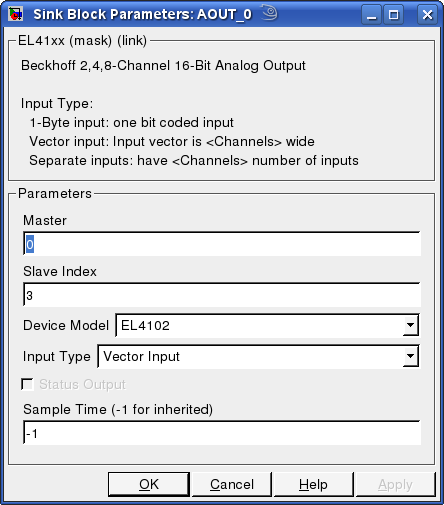
\includegraphics[width=0.4\textwidth]{images/el41xx.png}
    \caption{EL41xx configuration dialog}
    \label{fig:el41xx}
  \end{center}
\end{figure}

Figure~\ref{fig:el5001} shows the configuration dialog for the SSI
slave Beckhoff EL5001.

\begin{figure}[H]
  \begin{center}
    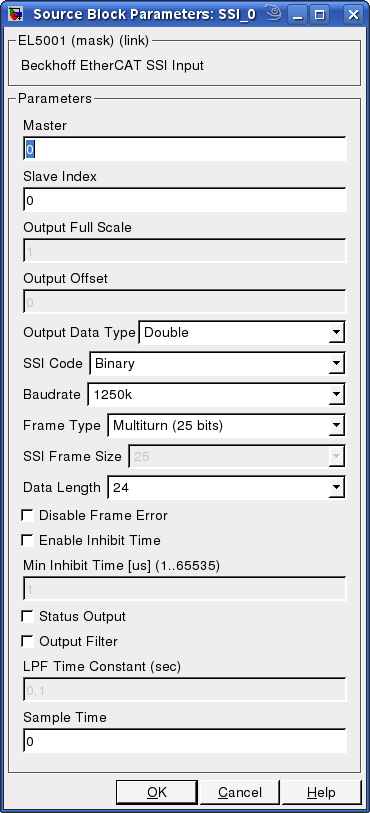
\includegraphics[width=0.4\textwidth]{images/el5001.png}
    \caption{EL5001 configuration dialog}
    \label{fig:el5001}
  \end{center}
\end{figure}

Figure~\ref{fig:el5101} shows the configuration dialog for the
incremental-encoder slave Beckhoff EL5101.

\begin{figure}[H]
  \begin{center}
    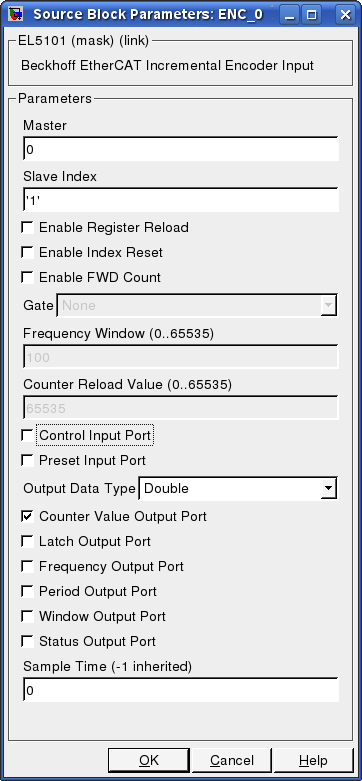
\includegraphics[width=0.4\textwidth]{images/el5101.png}
    \caption{EL5101 configuration dialog}
    \label{fig:el5101}
  \end{center}
\end{figure}

Figure~\ref{fig:bk1120-in} shows the configuration dialog for the Beckhoff
BK1120 KBUS-coupler input block.

\begin{figure}[H]
  \begin{center}
    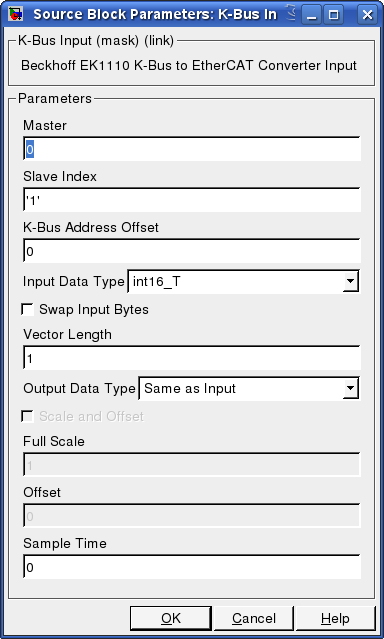
\includegraphics[width=0.4\textwidth]{images/bk1120-in.png}
    \caption{BK1120 input configuration}
    \label{fig:bk1120-in}
  \end{center}
\end{figure}

Figure~\ref{fig:bk1120-out} shows the configuration dialog for the Beckhoff
BK1120 KBUS-coupler output block.

\begin{figure}[H]
  \begin{center}
    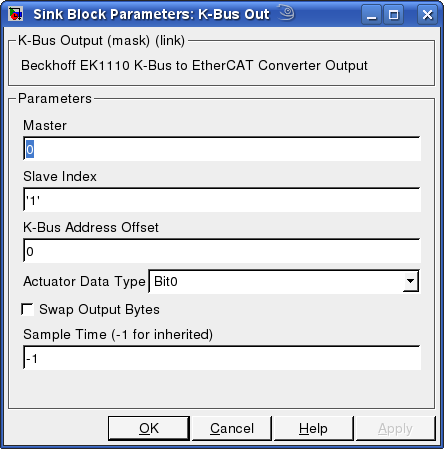
\includegraphics[width=0.4\textwidth]{images/bk1120-out.png}
    \caption{BK1120 output configuration}
    \label{fig:bk1120-out}
  \end{center}
\end{figure}

Figure~\ref{fig:masterstats} shows the configuration dialog for the EtherCAT
master status block.

\begin{figure}[H]
  \begin{center}
    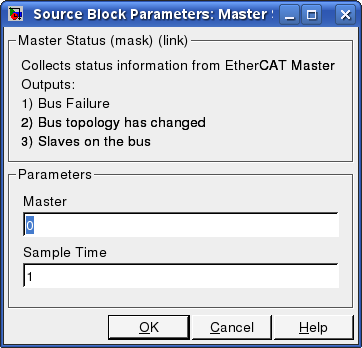
\includegraphics[width=0.4\textwidth]{images/master.png}
    \caption{Master status block configuration}
    \label{fig:masterstats}
  \end{center}
\end{figure}

\end{ighsec}

%--------------------------------------------------------------------

\begin{ighsec}{Creation of EtherLab\regTM\ Models}
\label{sec:modelle}

After creating a new model sheet within Simulink, a few parameters have to be
set up (menu \textit{Simulation/Configuration Parameters\ldots}):

\begin{itemize}
\item The input field \textit{Realtime Workshop} $\rightarrow$
  \textit{System target file} must contain the file name
  \texttt{etherlab.tlc}. It can be chosen via the
  \textit{Browse\ldots} button (see figure~\ref{fig:konfiguration}).
  \begin{figure}[H]
    \begin{center}
      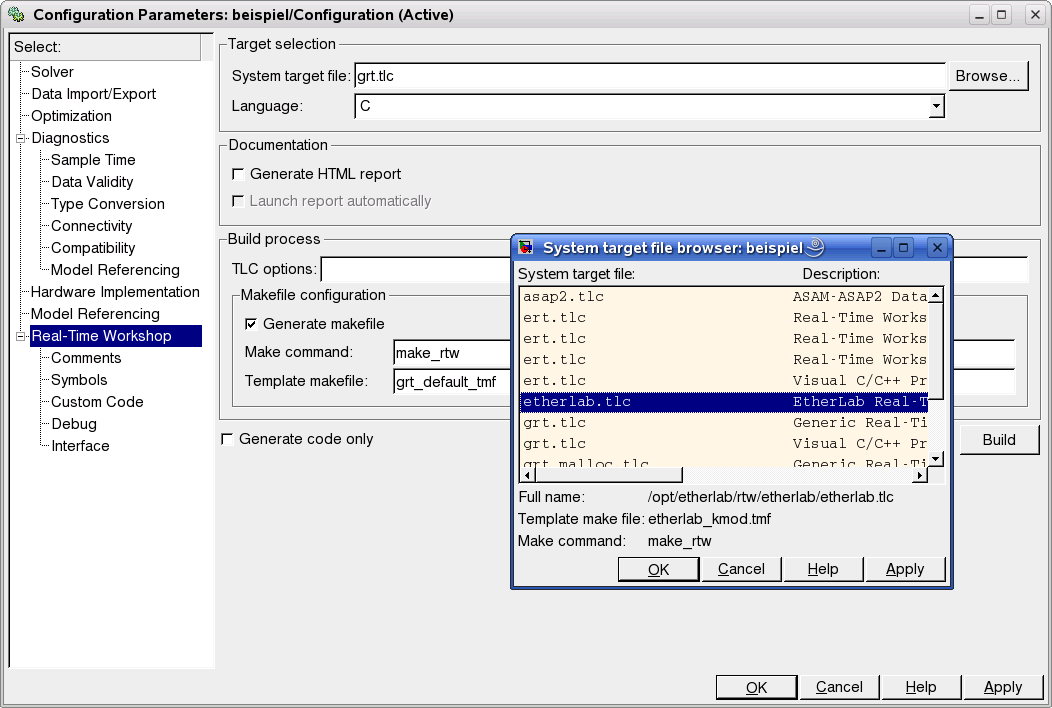
\includegraphics[width=.9\textwidth]{images/config_param.png}
      \caption{Configuration of model parameters}
      \label{fig:konfiguration}
    \end{center}
  \end{figure}
\item The input field \textit{Solver} $\rightarrow$ \textit{Fixed-step
    size} must contain the period time of the real time cycle, for
  example \texttt{0.01} meaning $100$ Hz (see
  figure~\ref{fig:config_solver}).
  \begin{figure}[H]
    \begin{center}
      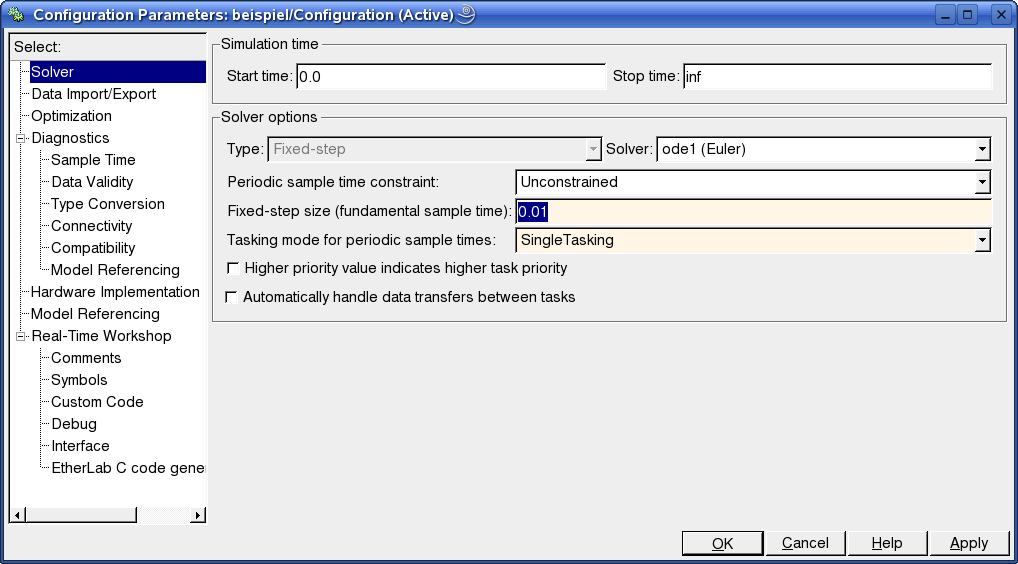
\includegraphics[width=.9\textwidth]{images/config_solver.png}
      \caption{Configuration of model parameters (2)}
      \label{fig:config_solver}
    \end{center}
  \end{figure}
\end{itemize}

After the model has been parametrized, it can be edited as usual. To use
EtherLab blocks, open the \texttt{etherlab\_lib} (see sec.~\ref{sec:lib}) and drag the
desired blocks on the new model sheet. When finished, \textit{Ctrl-B} will
generate the model code including a Linux kernel module.

\end{ighsec}

%--------------------------------------------------------------------

\begin{ighsec}{Starting of EtherLab\regTM\ Models}
\label{sec:start}

The \texttt{rt\_kernel} module must be inserted before inserting any
EtherLab\regTM\ modules. If EtherLab\regTM/RTW is configured as a
service (see section~\ref{sec:dienst}), this is done automatically at
system startup. Otherwise the module can be inserted manually. It is
recommended to start the module using the init script, because the
necessary device files are then created automatically:

\begin{lstlisting}
  # `\textbf{/opt/etherlab/rtw/bin/etherlab start}`
\end{lstlisting}

After that, an EtherLab\regTM/RTW module can be loaded and the buddy process
can be started, to exchange process data with user space programs (like
EtherLab Testmanager, EtherLab DLS, \ldots). Therefore the
\texttt{etherlab\_buddy} acts as a TCP server listening on port 2345 and
communicating with an XML-based protocol called MSR (see the german
documentation at \url{http://etherlab.org/download/m-igh_rt_api.pdf}).

\begin{lstlisting}
  # `\textbf{insmod <model>\_kmod.ko}`
  # `\textbf{/opt/etherlab/rtw/bin/etherlab\_buddy}`
\end{lstlisting}

If the \texttt{insmod} command returns with an error, the kernel ring
buffer can be analyzed for possible software or hardware
misconfigurations:

\begin{lstlisting}
  # `\textbf{dmesg}`
\end{lstlisting}

\end{ighsec}

%--------------------------------------------------------------------
%%% Local Variables:
%%% mode: latex
%%% TeX-master: "m-etherlab_rtw"
%%% End:


%
% der Index (in Vorbereitung 10/2004)
%\ighindex
%

% das Literaturverzeichnis (in Vorbereitung 10/2004)
%\ighbib
%

\end{document}

%%% Local Variables:
%%% mode: latex
%%% TeX-master: t
%%% End:
